% !TeX program = lualatex
% Vector illustrations for the SlideMage manual (example/decks/slidemage-manual.tex).
% One page per illustration; tools/manual/make_illustrations.py compiles this
% file and splits the pages into example/media/:
%   page 1  illustration-slidemage-splash.pdf     16:9, the \fullbleedframe demo
%   page 2  illustration-slide-stack-portrait.pdf  portrait, sideimageframe and
%                                                   \sectionfigure demos
%   page 3  chapter-logo-building-blocks.pdf       square icon, \chapterlogo demo
% Colors: the SlideMage template's palette (latex/Slidemaster_preamble_slidemage.tex).
\documentclass[tikz,border=0pt]{standalone}
\usepackage{fontspec}
\setmainfont{FiraSans-Regular.otf}[BoldFont=FiraSans-SemiBold.otf]
\definecolor{smdark}{HTML}{1e1e1e}
\definecolor{smblue}{HTML}{0066cc}
\definecolor{smlightblue}{HTML}{9ec7f0}
\definecolor{smyellow}{HTML}{ffd500}
\definecolor{smgray}{HTML}{e4e4e4}
\definecolor{smmid}{HTML}{6f6f6f}

% One slide card: #1 = name of its lower-left corner, size 4.8 x 2.7.
\newcommand{\slidecard}[2][]{%
	\begin{scope}[shift={#2}, #1]
		\fill[white, draw=smmid, line width=0.6pt, rounded corners=1.5pt] (0,0) rectangle (4.8,2.7);
		\fill[smdark, rounded corners=1.5pt] (0,2.15) rectangle (4.8,2.7);
		\fill[smdark] (0,2.15) rectangle (4.8,2.4);
		\fill[white] (0.25,2.33) rectangle (2.4,2.47);
		\fill[smdark] (0,0) rectangle (4.8,0.14);
		\foreach \y/\w in {1.75/3.6, 1.35/3.0, 0.95/3.4, 0.55/2.2} {
			\fill[smblue] (0.4,\y) circle (0.07);
			\fill[smmid] (0.65,\y-0.04) rectangle (0.65+\w,\y+0.04);
		}
		\fill[white, draw=smmid, line width=0.4pt] (4.2,2.18) rectangle (4.7,2.67);
		\fill[smyellow] (4.45,2.425) circle (0.13);
	\end{scope}%
}

\begin{document}

% 1 -- splash, 16:9
\begin{tikzpicture}
	\fill[smdark] (0,0) rectangle (16,9);
	\node at (8,5.4) {\includegraphics[width=4.2cm]{slidemage-logo.pdf}};
	\node[text=white, font=\bfseries\fontsize{40}{44}\selectfont] at (8,2.95) {SlideMage};
	\fill[smyellow] (6.6,2.05) rectangle (9.4,2.2);
	\node[text=smgray, font=\fontsize{15}{18}\selectfont] at (8,1.25) {Slides as building blocks};
\end{tikzpicture}

% 2 -- a stack of slides, portrait
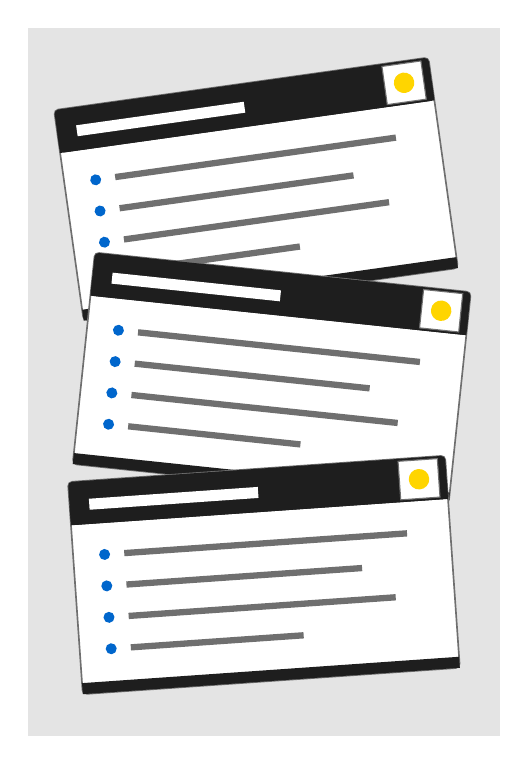
\begin{tikzpicture}
	\fill[smgray] (0,0) rectangle (6,9);
	\slidecard[rotate around={8:(2.4,1.35)}]{(0.5,5.6)}
	\slidecard[rotate around={-6:(2.4,1.35)}]{(0.7,3.2)}
	\slidecard[rotate around={4:(2.4,1.35)}]{(0.6,0.7)}
\end{tikzpicture}

% 3 -- chapter logo: building blocks

\begin{tikzpicture}
	\useasboundingbox (0,0) rectangle (3,3);
	\fill[smblue, rounded corners=2pt] (0.05,0.05) rectangle (1.45,1.45);
	\fill[smdark, rounded corners=2pt] (1.55,0.05) rectangle (2.95,1.45);
	\fill[smyellow, rounded corners=2pt] (0.8,1.55) rectangle (2.2,2.95);
\end{tikzpicture}

\end{document}
